\begin{problem}{/images/problems/20_marbles.jpg}{Bag of Pebbles}
	You take part in a game wherein there is a bag with 1000 black pebbles and 1000 white pebbles. Each time, you can randomly pick a pebble from the bag and remove it. If the removed pebble is black, you will receive one dollar and if it is white, you will be fined one dollar. You can continue the game as long as there is at least one pebble in the bag and stop the game at any point you wish. How would you play in this game and what is your expected reward? (The optimal strategy requires a lot of complex calculations which cannot be done without a computer. The goal of the question is to find a strategy that is simple and almost optimal.)\\[0.2cm]

Link to the problem on Twitter:  \url{https://twitter.com/Riazi_Cafe/status/1687349831696809984}
\end{problem}
\begin{solution}.
As mentioned, the goal of the problem is not to find the optimal strategy, and therefore there are different answers to the question. Our proposed algorithm is to continue the game until the number of remaining white pebbles is greater than the number of remaining black pebbles plus the square root of the number of remaining black pebbles. In this case, our average reward is equal to 16.224, which is more than $98\%$ of the highest possible reward achievable with any strategy.\\[0.2cm]

First, we discuss what we should expect of the reward of the optimal strategy. Notice that in any case, if we continue the game until the bag is empty, our net reward will be 0, so we never leave the game with a negative reward. Intuitively, if we flip a coin $n$ times, the expectation of the difference between the number of heads and the number of tails will be close to $\sqrt{n}$ (up to a constant multiplicative factor). Therefore, we do not expect the optimal strategy to  achieve an asymptotically higher reward than $O(\sqrt{n})$ in expectation. 


We first explain two types of strategies that were proposed in the comments:

\begin{itemize}
\item The first strategy is to continue the game until our total reward reaches a certain number or we remove all of the pebbles from the bag. This method gives us a good approximation of the optimal reward. In the plot below, you can see what our average reward would be for any specific threshold. The maximum reward we can get with this method is equal to 13.56, which is obtained with a threshold of 22. This amounts to about $82\%$ of the optimal reward.

\begin{center}
	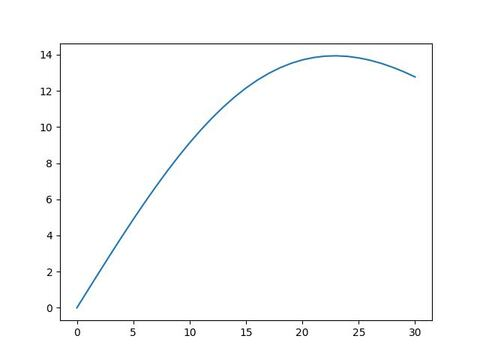
\includegraphics{/images/problems/20_diagram1.jpg}
\end{center}

\item The second strategy is to continue the game for $n$ steps. if our total reward is positive after $n$ steps, we stop there, otherwise, we continue the game until the end. In this case, the plot below shows our average reward for any $n$. The maximum average reward we can obtain with this strategy is for the case of $n=1000$ which guarantees a reward of $8.92$ for us on average. This value is about $54\%$ of the optimal reward.

\begin{center}
	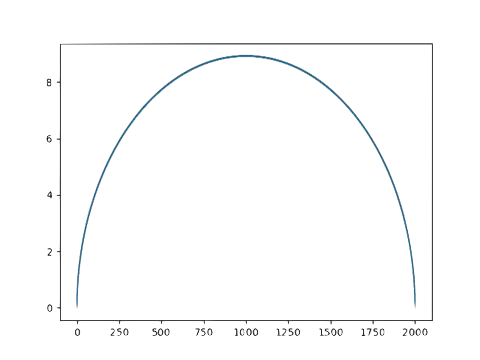
\includegraphics{/images/problems/20_diagram2.jpg}
\end{center}
\end{itemize}


The intuition behind our proposal is that the most important factor to determine whether to stop or not is how much the number of remaining white balls  is greater than the number of remaining black balls . As discussed above, the stopping rule should compare the difference to the square root of the number of pebbles.

\end{solution}